\subsection{Manager View}

%For the main pages put a mockup and describe it in detail.

\begin{center}
    \frame{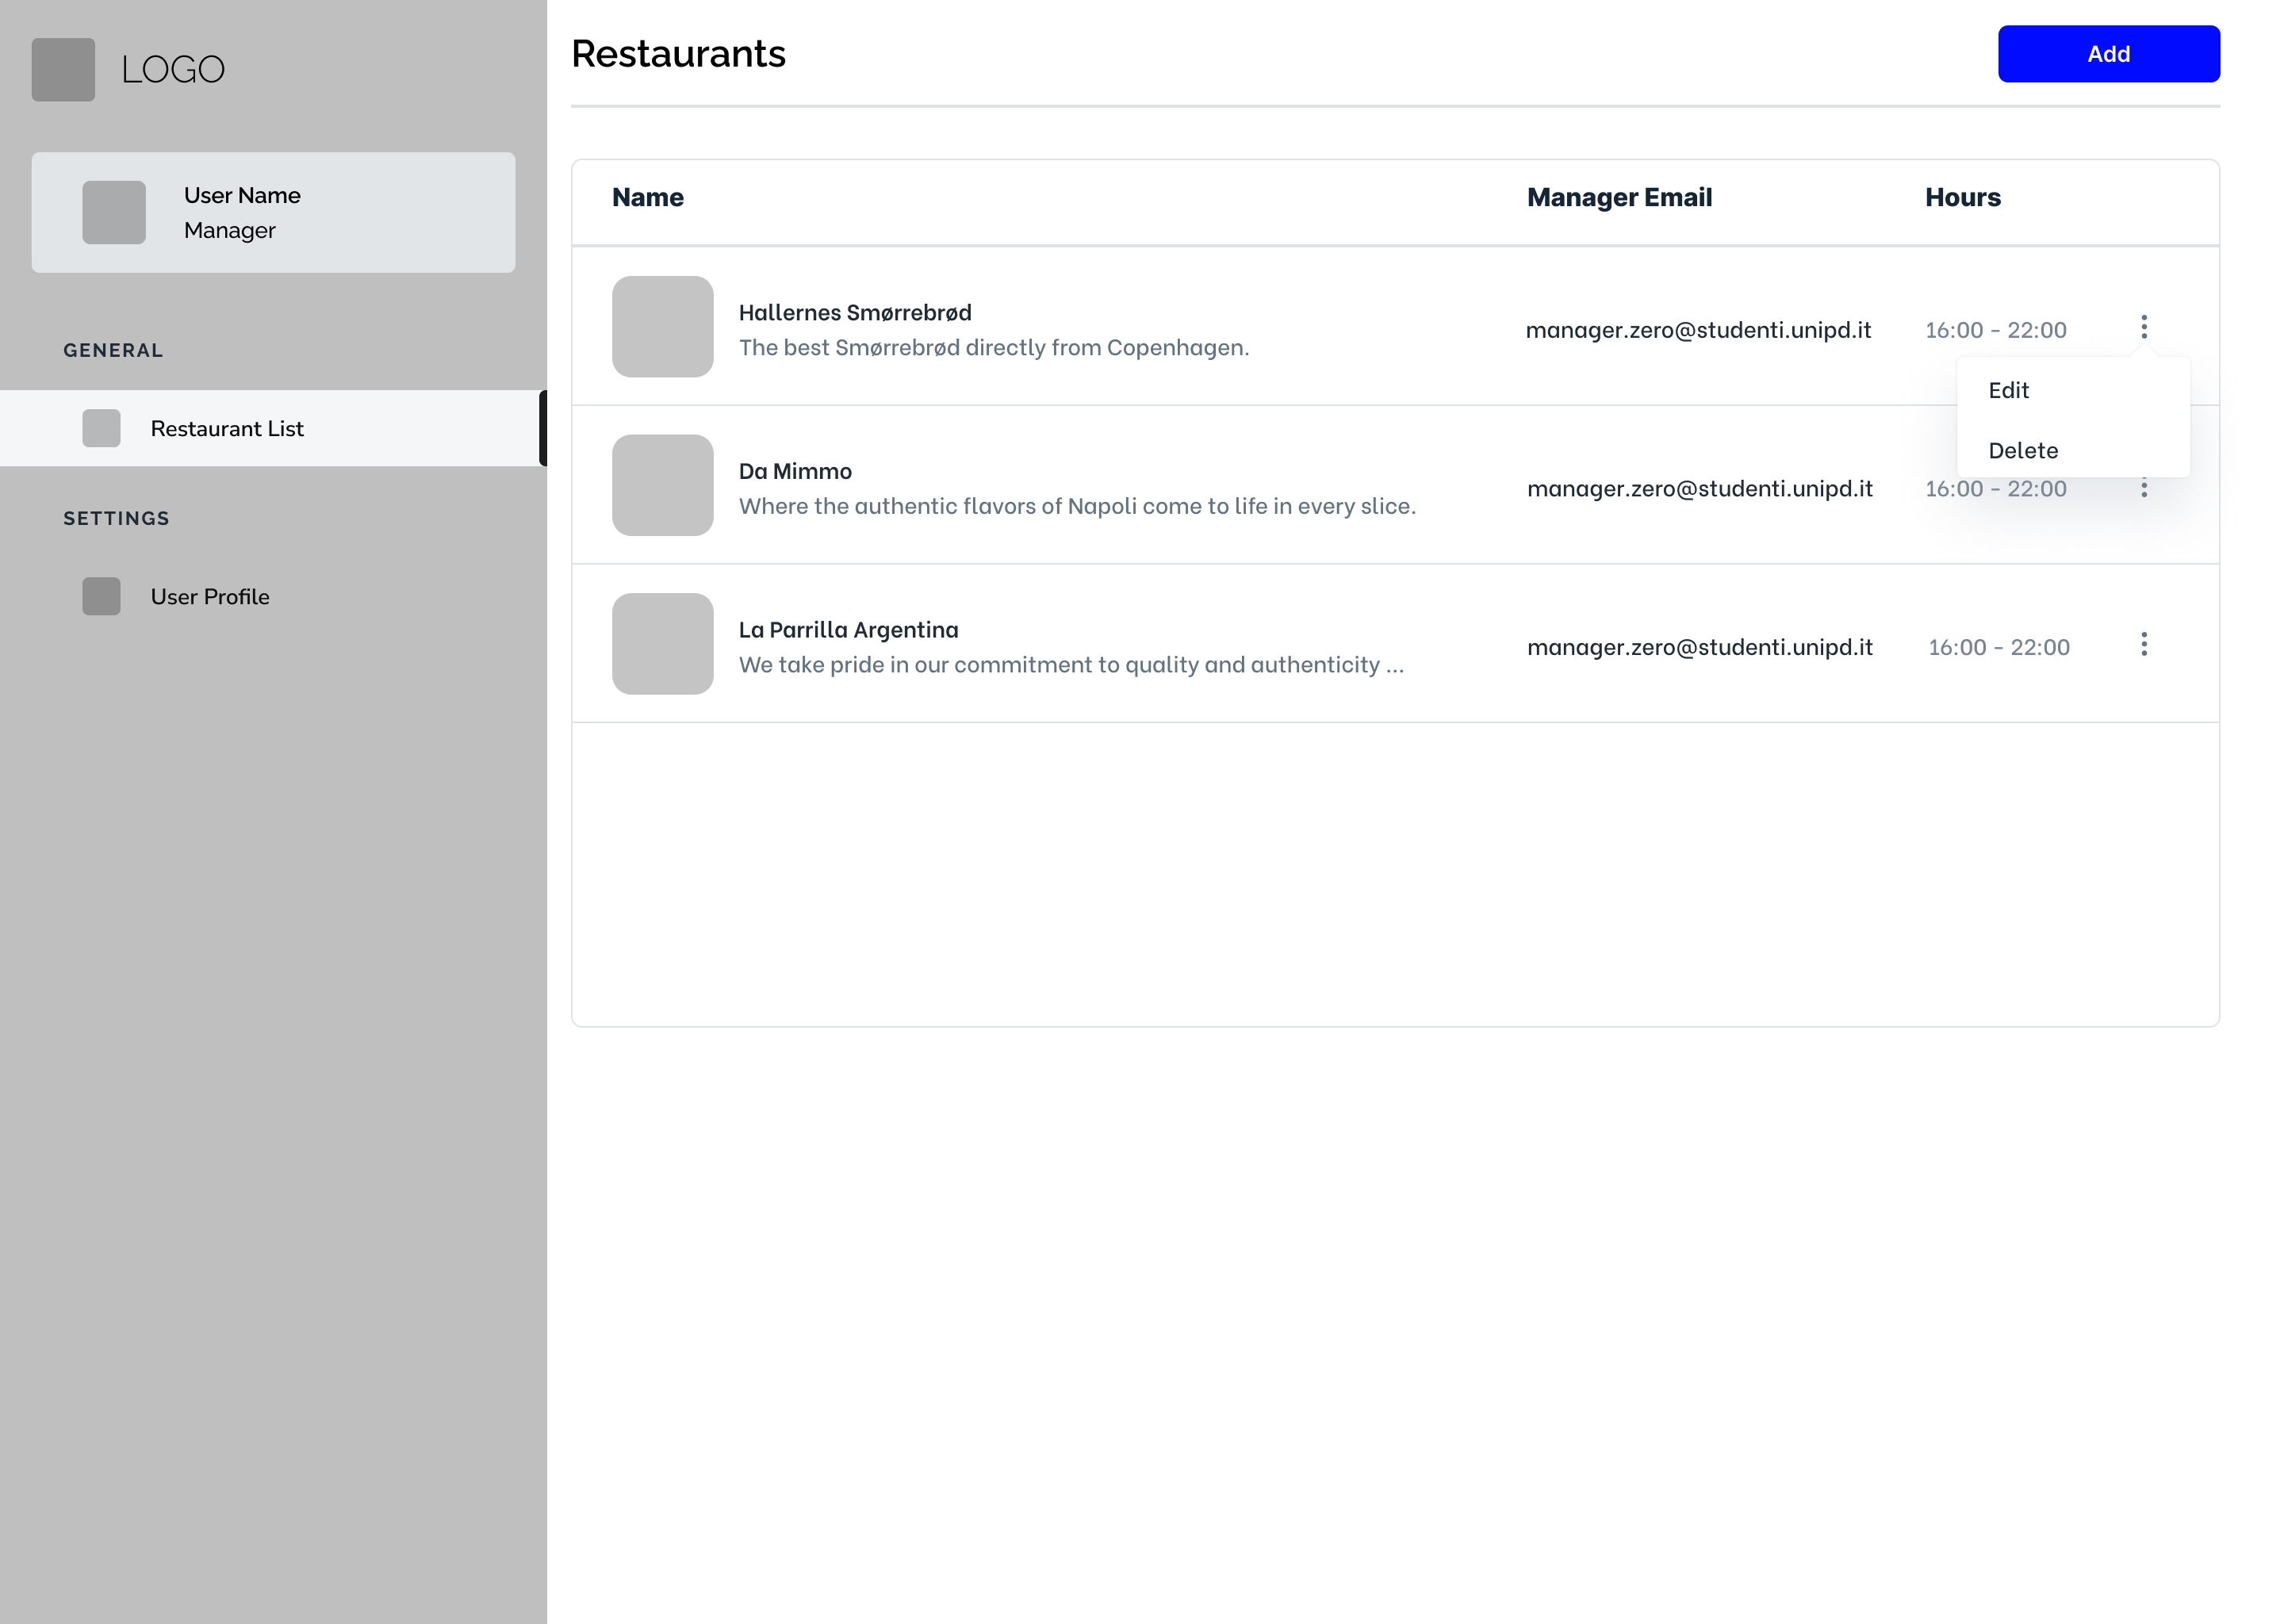
\includegraphics[width=.8\textwidth]{resources/mockup/admin/Admin-view-ListOfRestaurants-1.jpg}}
    \captionof{figure}{List of restaurants from manager view.}
    \label{fig:manager-ListOfRestaurants}
\end{center}

For the manager, we have a list of restaurants accessible when the manager is logged in, and the view is different for the user and manager, and only the manager can see it. As can be seen from the figure, the manager is able to edit and delete a restaurant from the list. For editing, the user will be directed to the form for the restaurant details and data of the restaurants, such as the description of each restaurant, the manager's email, and the opening and closing hours.



\begin{center}
    \frame{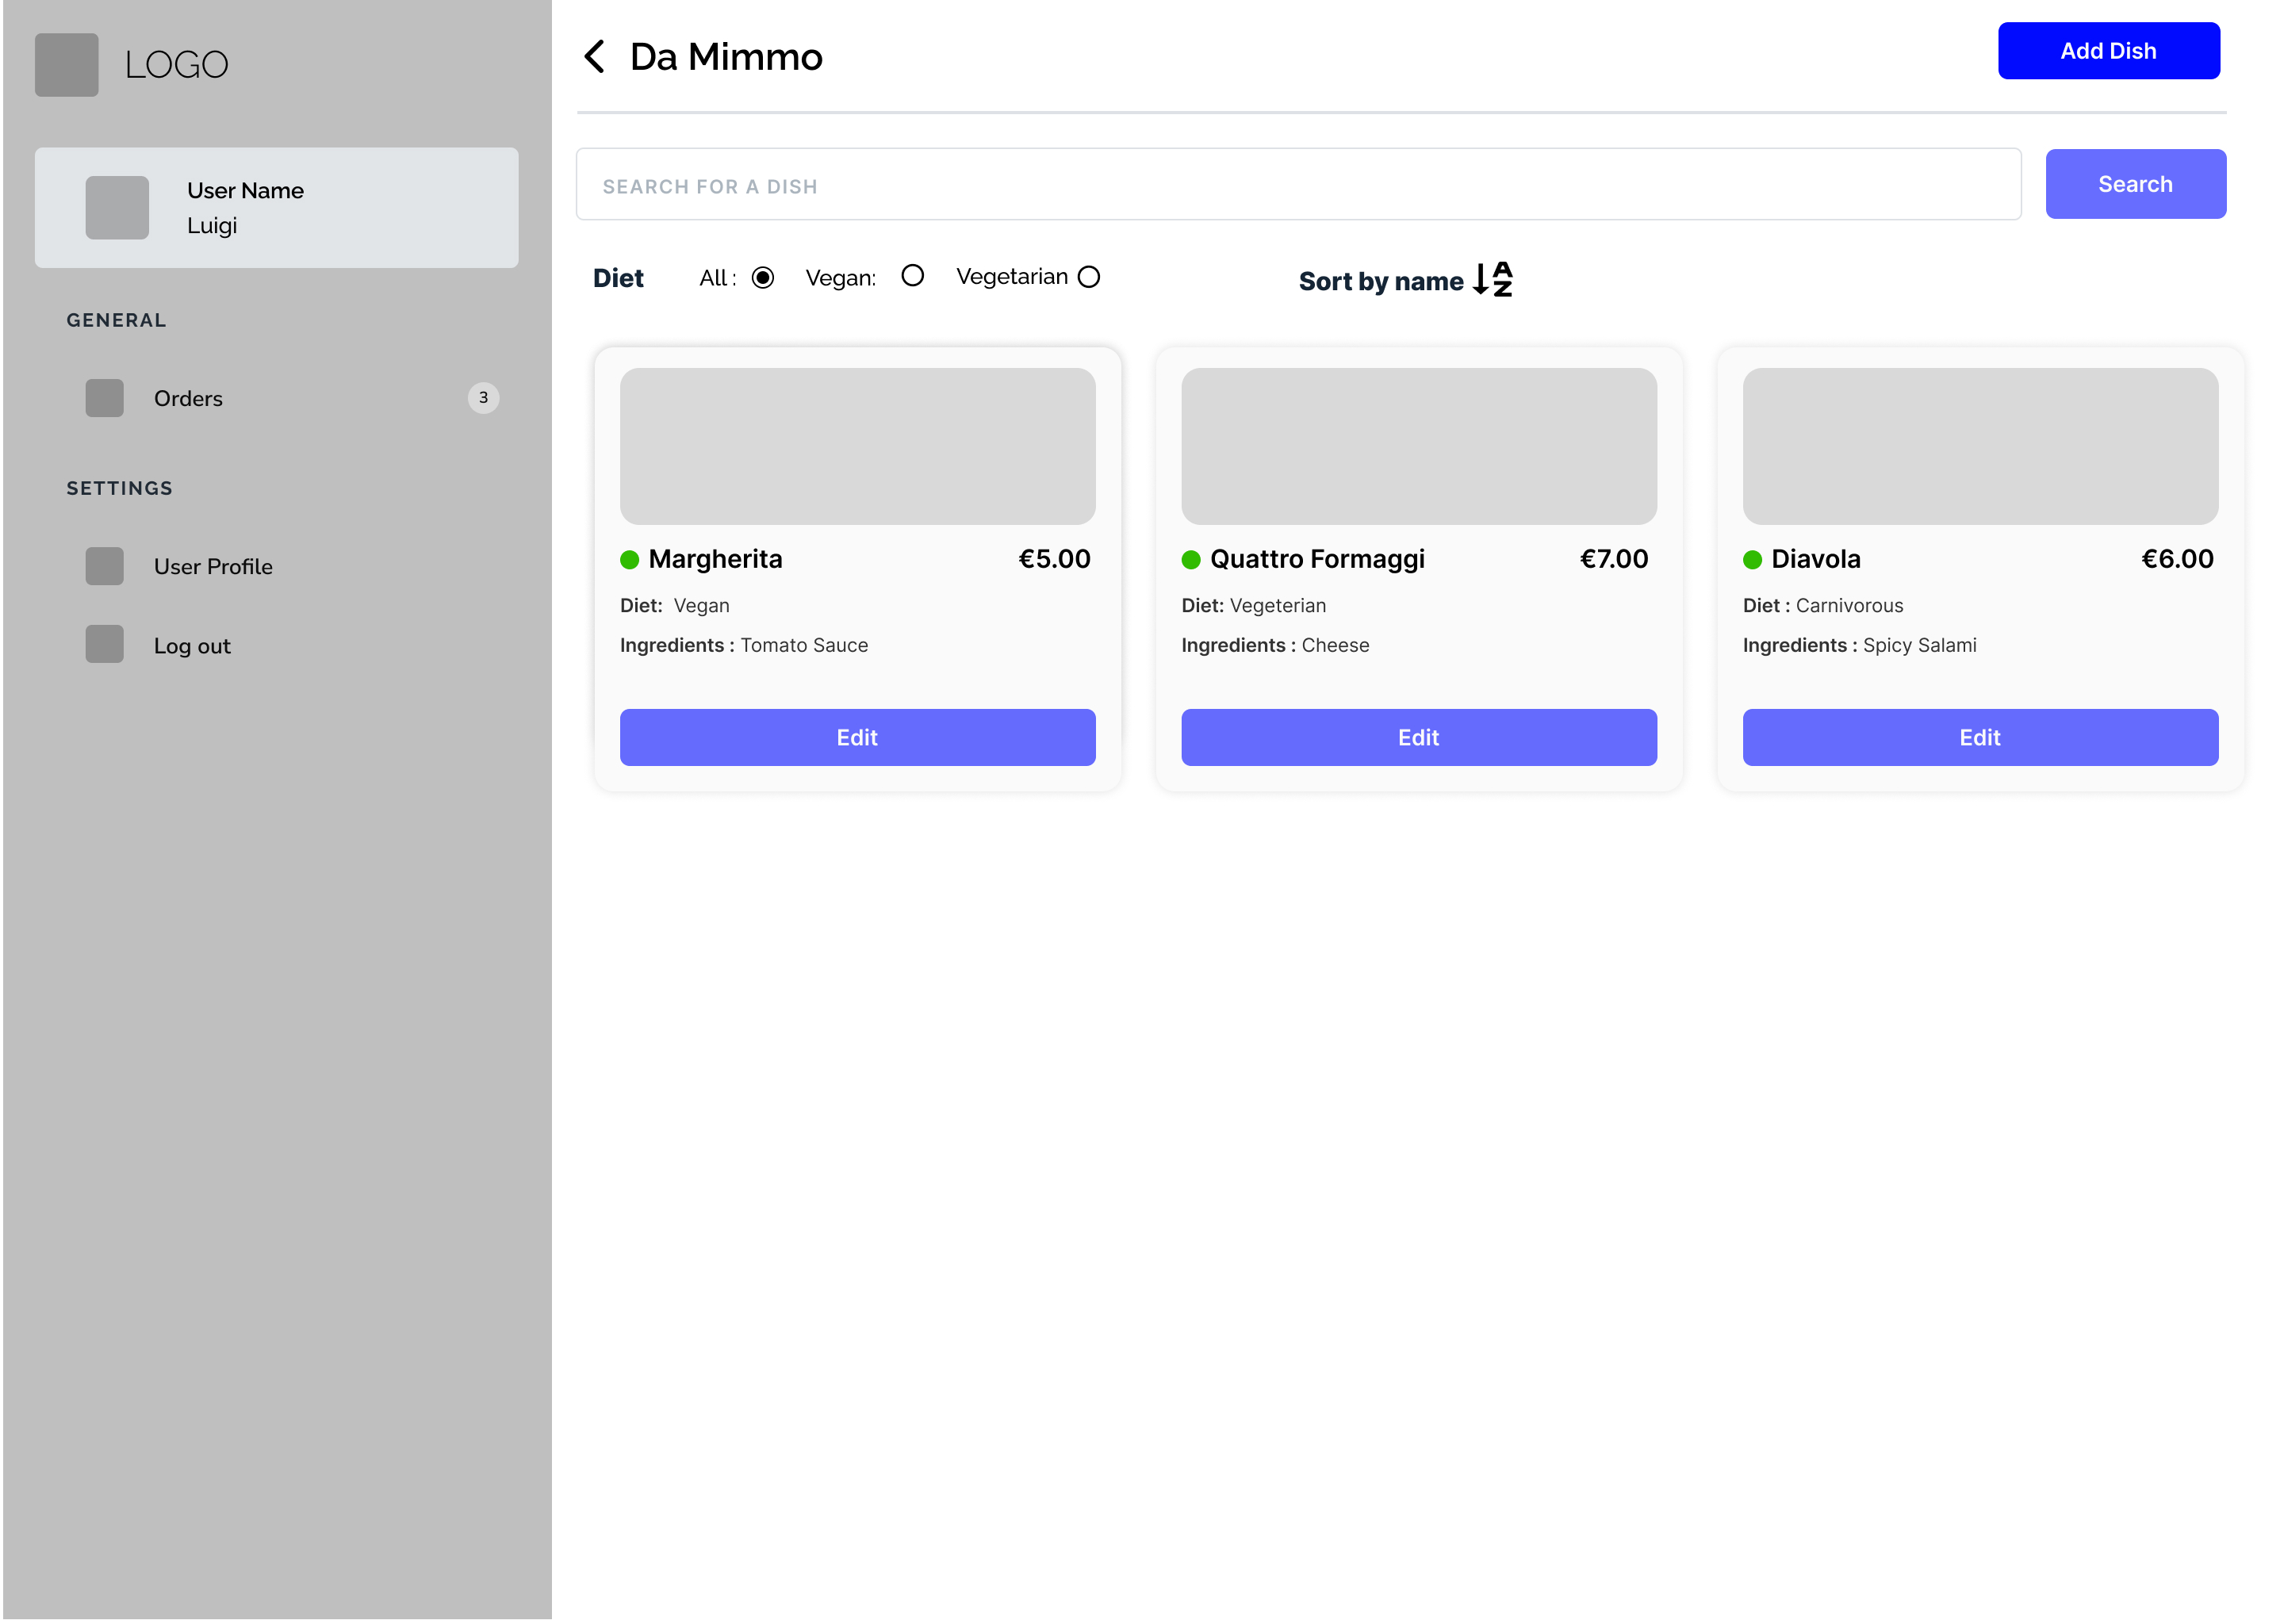
\includegraphics[width=.8\textwidth]{resources/mockup/admin/Admin-dish-list.jpg}}
    \captionof{figure}{List of dishes from manager view.}
    \label{fig:manager-ListOfRestaurants}
\end{center}

The manager is able to view all the dishes and also make changes to each dish. This is included with the availability of adding and removing dishes. It is also feasible that both the administrator and manager have access to the dishes and can modify them. As you can see from Figure 11, there is also a feature for adding dishes. You will be directed to the form for adding the dish, and you will be able to edit the name, price, ingredients, and other attributes of the dish.